% This is a most basic header

% article with standard layout
\documentclass[12pt,a4paper]{article}

%encoding text
\usepackage[utf8]{inputenc}
\usepackage[english]{babel}

%fond
\usepackage[T1]{fontenc}
\usepackage{upgreek}

% math formulas
\usepackage{amsmath}
\usepackage{amsfonts}
\usepackage{amssymb}
\usepackage{amsthm}		% theorem environments

% math fond
\usepackage{fourier}

%graphics
\usepackage{graphicx}


%layout
\setlength{\parindent}{0pt}



\newcommand{\td}{\ensuremath{\text{d}} }


\newcommand{\tab}[1]{\ensuremath{\quad \text{#1} \quad}}
\newcommand{\e}{\ensuremath{\text{e}}}

\newcommand{\adj}[1]{\ensuremath{ \, \text{adj}\,#1 \,\, }}
\renewcommand{\det}[1]{\ensuremath{ \, \text{det}\,#1 \,\, }}
\newcommand{\rank}[1]{\ensuremath{ \, \text{rank}\,#1 \,\, }}
\newcommand{\kernel}[1]{\ensuremath{ \, \text{kernel}\,#1 \,\,}}
\renewcommand{\dim}[1]{\ensuremath{ \, \text{dim}\,#1 \,\,}}
\newcommand{\linspan}[1]{\ensuremath{ \, \text{span}\,#1 \,\,}}
\newcommand{\supremum}[2]{\ensuremath{ \, \underset{#2}{\text{sup}}\,#1 \,\,}}


\begin{document}



\section{Parameter-Tuning}
Given a $\mathbf{R}^n$ nominal system ($u$ not written)
\begin{align}
\frac{\td x}{\td t} = f(x)
\end{align}
with initial values $x(0) = x_0 \in \mathbb{R}^n$ an $t\in [0,T]$ and measuring function 
$h(x) = y \in \mathbb{R}^m$, a dataset
\begin{equation}
\mathcal{D} = \left\{ (t[1],y[1]), (t[2],y[2]),\ldots , (t[N],y[N]) \right\}
\end{equation}
and the dynamic elastic net approach
\begin{equation}
\hat{f}(\hat{x},w) = f(\hat{x}) + w \label{eq:dynelnet}
\end{equation}


the cost-functional is
\begin{equation}
J[w] = \sum\limits_{\mathcal{D}} || y - h(\hat{x}) ||_Q^2 + \mathcal{R}[w] \quad ,
\end{equation}
where $\hat{x}$ solves \eqref{eq:dynelnet}. The matrix $Q$ is the weight matrix 
and 
\begin{equation}
\mathcal{R}[w] = \alpha_1 ||w||_1 + \frac{\alpha_2}{2} ||w||_2^2
\end{equation}
is the regularisation term.



\section{Cascade-Model}
Nominal model with statespace $\mathbb{R}^4$, measure function $h(x) = x$ 
and time interval $[0,T]$. Dependence of $x$ and $u$ on $t$ not written. The initial 
values are $x(0)=0$.

\begin{align}
f(x) &=
\left[ \underbrace{
\begin{pmatrix}
0 & 0 & 0 & 0 \\
\beta_1 & 0 & 0 & 0 \\
 0& \beta_2  & 0 & 0 \\
0& 0 & \beta_3  & 0 
\end{pmatrix} }_\text{cascade}
+
\underbrace{
\begin{pmatrix}
- \gamma_1 & 0 & 0 & 0 \\
0 & - \gamma_2 &0 & 0 \\
0 & 0 & - \gamma_3 & 0 \\
0 & 0 & 0 & - \gamma_4
\end{pmatrix} }_\text{self-loops}
\right]
\begin{pmatrix}
x_1 \\ x_2 \\ x_3 \\ x_4
\end{pmatrix}
+
\begin{pmatrix}
1 \\ 0 \\ 0 \\ 0 
\end{pmatrix}
u \\
&= \left[ A_1 + A_2 \right] x + Bu
\quad .
\end{align}
Using the general solution 
\begin{equation}
x(t) = \int\limits_0^t \text{e}^{(A_1+A_2)(t-\tau)}
B u (\tau) \td \tau
\end{equation}
and with $t- \tau \to \tau  $, $u( t - \tau) := u(\tau)$ and 
$\alpha_i = \alpha$, $\beta_i = \beta$ for simplicity
we get
\begin{equation}
x_n(t) = \int\limits_0^t e^{-\alpha\tau} b^{n-1}\frac{\tau^{n-1}}
{(n-1)!} u(\tau) \td \tau
\end{equation}

\begin{figure}[h]
	\centering
	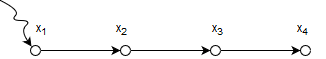
\includegraphics[scale=0.8]{graphics/cascade1.png}
\end{figure}

Here we will use 
\begin{equation}
u(t) = \frac{a}{2 \omega} \sin(\omega t)\cos(\omega t) \quad .
\end{equation}
thus we get
\begin{align}
x_1(t) = \frac{(1 - \e^{-\alpha t})}{\alpha}  
\end{align}
\subsection{$\delta$-peak}
Delta-peaks are regularly used in electrical-engineering and as a mathematical tool in 
the theory of partial differential equations.\\

Perturbation function with $\mathcal{N} > 0$, $\Gamma > 0$, $t_0 \in (0,T)$
\begin{equation}
\delta(t) = \begin{cases}
& \mathcal{N} (2 \Gamma)^{-1} \quad \text{if} \quad t_0 -\Gamma \leq t \leq t_0 + \Gamma \\
& 0 \quad \text{else}
\end{cases}
\end{equation}
and perturbed system.
\begin{align}
f^\delta(x,t) = f(x) + \begin{pmatrix}
0 , 0 , \delta(t) , 0
\end{pmatrix}^\text{T} \quad .
\end{align}

\subsection{Breit-Wigner-Resonance}
The Breit-Wigner-resonance is the standard resonance curve in classical an quantum 
mechanics and also known as Cauchy-distribution (statistics) and Lorentz-curve 
(spectroscopy).\\

Perturbation function
\begin{equation}
F(t) = \mathcal{N} \uppi^{-1} \frac{\Gamma}{\Gamma^2 + (t-t_0)^2}
\end{equation}
and perturbed system
\begin{equation}
f^F(x,t) = f(x) +\begin{pmatrix}
0, 0, F(t) , 0
\end{pmatrix}^\text{T} \quad . 
\end{equation}


\section{Chaotic Systems}
\subsection{Lorentz-System}
The nominal model is in $\mathbb{R}^3$, measure function $h(x)=x$ and $a,b,c>0$. 
\begin{equation}
f(x) = \begin{pmatrix}
a (y-x) \\ bx -y -yz \\ xy - z
\end{pmatrix}
\end{equation}
\subsection{Verhulst-Dynamic}
A simple chaotic model, also known as logistic growth curve, with interesting behaviour 
when $r \sim 3.57$.
\begin{equation}
f(x) = rx(1-x) \quad .
\end{equation}

\section{Oscillations}
\subsection{harmonic oscillator}
\begin{equation}
\ddot{x} + \omega^2 x = 0
\end{equation}


\end{document}